\documentclass[xcolor={dvipsnames}]{beamer}
%\usepackage[utf8]{inputenc}
\usetheme{Madrid}
%\usetheme{Malmoe}
\usecolortheme{beaver}
%\usecolortheme{rose}

%-------------------------------------------------------------------------------
%          -Packages nécessaires pour écrire en Français et en UTF8-
%-------------------------------------------------------------------------------
\usepackage[utf8]{inputenc}
\usepackage[frenchb]{babel}
\usepackage[T1]{fontenc}
\usepackage{lmodern}
\usepackage{textcomp}

%-------------------------------------------------------------------------------

%-------------------------------------------------------------------------------
%                          -Outils de mise en forme-
%-------------------------------------------------------------------------------
\usepackage{hyperref}
\hypersetup{pdfstartview=XYZ}
\usepackage{enumerate}
\usepackage{graphicx}
%\usepackage{multicol}
%\usepackage{tabularx}

%\usepackage{anysize} %%pour pouvoir mettre les marges qu'on veut
%\marginsize{2.5cm}{2.5cm}{2.5cm}{2.5cm}

\usepackage{indentfirst} %%pour que les premier paragraphes soient aussi indentés
\usepackage{verbatim}
%\usepackage[table]{xcolor}  
%\usepackage{multirow}
\usepackage{ulem}
%-------------------------------------------------------------------------------


%-------------------------------------------------------------------------------
%                  -Nécessaires pour écrire des mathématiques-
%-------------------------------------------------------------------------------
\usepackage{amsfonts}
\usepackage{amssymb}
\usepackage{amsmath}
\usepackage{amsthm}
\usepackage{tikz}
\usepackage{xlop}
\usepackage[output-decimal-marker={,}]{siunitx}
%-------------------------------------------------------------------------------


%-------------------------------------------------------------------------------
%                    - Mise en forme 
%-------------------------------------------------------------------------------

\newcommand{\bu}[1]{\underline{\textbf{#1}}}


\usepackage{ifthen}


\newcommand{\ifTrue}[2]{\ifthenelse{\equal{#1}{true}}{#2}{$\qquad \qquad$}}

\newcommand{\kword}[1]{\textcolor{red}{\underline{#1}}}


%-------------------------------------------------------------------------------



%-------------------------------------------------------------------------------
%                    - Racourcis d'écriture -
%-------------------------------------------------------------------------------

% Angles orientés (couples de vecteurs)
\newcommand{\aopp}[2]{(\vec{#1}, \vec{#2})} %Les deuc vecteurs sont positifs
\newcommand{\aopn}[2]{(\vec{#1}, -\vec{#2})} %Le second vecteur est négatif
\newcommand{\aonp}[2]{(-\vec{#1}, \vec{#2})} %Le premier vecteur est négatif
\newcommand{\aonn}[2]{(-\vec{#1}, -\vec{#2})} %Les deux vecteurs sont négatifs

%Ensembles mathématiques
\newcommand{\naturels}{\mathbb{N}} %Nombres naturels
\newcommand{\relatifs}{\mathbb{Z}} %Nombres relatifs
\newcommand{\rationnels}{\mathbb{Q}} %Nombres rationnels
\newcommand{\reels}{\mathbb{R}} %Nombres réels
\newcommand{\complexes}{\mathbb{C}} %Nombres complexes


%Intégration des parenthèses aux cosinus
\newcommand{\cosP}[1]{\cos\left(#1\right)}
\newcommand{\sinP}[1]{\sin\left(#1\right)}

%Fractions
\newcommand{\myfrac}[2]{{\LARGE $\frac{#1}{#2}$}}

%Vocabulaire courrant
\newcommand{\cad}{c'est-à-dire}

%Droites
\newcommand{\dte}[1]{droite $(#1)$}
\newcommand{\fig}[1]{figure $#1$}
\newcommand{\sym}{symétrique}
\newcommand{\syms}{symétriques}
\newcommand{\asym}{axe de symétrie}
\newcommand{\asyms}{axes de symétrie}
\newcommand{\seg}[1]{$[#1]$}
\newcommand{\monAngle}[1]{$\widehat{#1}$}
\newcommand{\bissec}{bissectrice}
\newcommand{\mediat}{médiatrice}
\newcommand{\ddte}[1]{$[#1)$}

%Figures
\newcommand{\para}{parallélogramme}
\newcommand{\paras}{parallélogrammes}
\newcommand{\myquad}{quadrilatère}
\newcommand{\myquads}{quadrilatères}
\newcommand{\co}{côtés opposés}
\newcommand{\diag}{diagonale}
\newcommand{\diags}{diagonales}
\newcommand{\supp}{supplémentaires}
\newcommand{\car}{carré}
\newcommand{\cars}{carrés}
\newcommand{\rect}{rectangle}
\newcommand{\rects}{rectangles}
\newcommand{\los}{losange}
\newcommand{\loss}{losanges}


%----------------------------------------------------


\usepackage{../../../../pas-math}
\usepackage{../../../../moncours_beamer}

\usepackage{amssymb,amsmath}


\newcommand{\myitem}{\item[\textbullet]}

\graphicspath{{../img/}}

\title{Séquence 3 : Fractions}
%\author{O. FINOT}\institute{Collège S$^t$ Bernard}

%
\AtBeginSection[]
{
	\begin{frame}
		\frametitle{}
		\tableofcontents[currentsection, hideallsubsections]
	\end{frame} 
	
}
%
%
%\AtBeginSubsection[]
%{
%	\begin{frame}
%		\frametitle{Sommaire}
%		\tableofcontents[currentsection, currentsubsection]
%	\end{frame} 
%}

\begin{document}
	
	
	
	\begin{frame}
		\titlepage 
	\end{frame}
	
	
	%	
	%
	%\begin{frame}
	%	\begin{block}{Objectifs}
	%		\begin{itemize}
	%			
	%			\item Savoir si deux fractions sont égales
	%			\item Savoir si un nombre est divisible par un autre
	%			\item Identifier un nombre premier
	%			\item Décomposer un nombre en produit de facteurs premiers
	%			\item Simplifier une fraction
	%			\item Comparer des fractions
	%			\item Additionner et soustraire des fractions dont les dénominateurs sont des multiples l’un de l’autre
	%			
	%			\end{itemize}
	%	\end{block}
	%\end{frame}
	%
	%\begin{frame}
	%	\begin{block}{Compétences travaillées}
	%		\begin{itemize}
	%			\item \kw{Représenter (Re2)} :  produire et utiliser plusieurs représentations d’un nombre;
	%			\item \kw{Calculer (Ca1)} :  calculer avec des nombres rationnels, de manière exacte ou approchée en combinant astucieusement le calcul mental, le calcul posé et le calcul instrumenté ;
	%			\item \kw{Raisonner (Ra1)} :  résoudre des problèmes impliquant des grandeurs variées : mobiliser les connaissances nécessaires, analyser et exploiter ses erreurs, mettre à l’essai plusieurs solutions.		
	%		\end{itemize}
	%	\end{block}
	%\end{frame}
	
	
	
	\section{Tableau de proportionnalité}
	
	\begin{frame}
		\begin{block}{Objectifs}
			\begin{itemize}
				\item reconnaître un tableau de proportionnalité
				\item Calculer un coefficient de proportionnalité
			\end{itemize}
		\end{block}
	
		\begin{block}{Compétence}
			\textbf{Modéliser} : J'identifie une situation de proportionnalité et je l'utilise pour résoudre un problème 
		\end{block}
	\end{frame}
	
	
	\begin{frame}
		\begin{mydefs}
		
			\begin{itemize}
				\item Un tableau a deux lignes est un \kword{tableau de proportionnalité} si on peut calculer les nombres de la deuxième lignes sont obtenues en multipliant ceux de la première \kword{par un même nombre}. \pause
				
				\item Ce nombre est le \kword{coefficient de proportionnalité}.\pause
			\end{itemize}			
			
		\end{mydefs}
	
		\begin{block}{Méthode} 
			Pour identifier une situation de proportionnalité, on calcule les quotients des nombres de la seconde ligne par ceux de la première ligne.\pause
			Il y a proportionnalité si c'est toujours le même.
		\end{block}
	\end{frame}

	\begin{frame}
		\begin{exampleblock}{Exemple}
			Ce tableau présente le prix de différentes masses de cerises :
			\begin{center}
				
				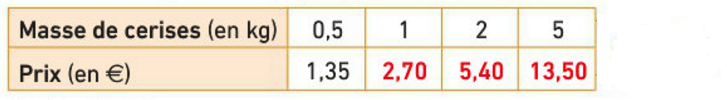
\includegraphics[scale=0.5]{tb_prop1-2}
			\end{center}
		\end{exampleblock}
	\end{frame}

	\begin{frame}
		\begin{exampleblock}{Exemple}
			Ce tableau présente le prix de différentes masses de cerises :
			\begin{center}
				
				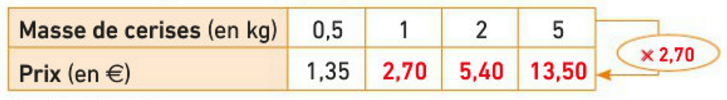
\includegraphics[scale=0.5]{tb_prop1}
			\end{center}
		
		$\num{1,35} \div \num{0.5} = \num{2,70} \div 1 = \num{5.40} \div 2 = \num{13,50} \div 5 = \num{2.70} $, ce tableau est un tableau de proportionnalité. \pause
		
		Le coefficient de proportionnalité est \num{2.70}.
		\end{exampleblock}
	\end{frame}
\end{document}